\documentclass[10pt,twocolumn]{article}
\usepackage[utf8]{inputenc}
\usepackage{geometry}
\geometry{a4paper, margin=1in}
\usepackage{booktabs}
\usepackage{graphicx}
\usepackage{amsmath}
\usepackage{hyperref}
\usepackage{microtype}

\title{\textbf{A Comparative Study of Dynamic Evidence Fusion in Scientific Document QA}}
\author{ScholAR Demonstration Team \\ \texttt{scholar-demo@example.org}}
\date{September 2026}

\begin{document}
\maketitle

\begin{abstract}
Answering complex questions from scientific literature demands precise evidence extraction across prose, quantitative tables, and visual figures. Standard document assistants frequently discard spatial grounding or treat figures as detached metadata. In this paper, we investigate Dynamic Evidence Fusion, a coordinate-aware retrieval and verification framework that unifies lexical search, dense embeddings, and rasterized bounding-box crops. On our benchmark evaluation, Dynamic Fusion achieves an F1 score of 88.4\% with an average retrieval latency of 42\,ms. Our findings demonstrate that preserving source identities and spatial coordinates significantly enhances factual grounding in scientific question answering.
\end{abstract}

\section{Introduction}
Scientific publications present structured knowledge where textual claims are tightly coupled with mathematical formulations, experimental tables, and visual diagrams. Existing retrieval-augmented generation systems often isolate plain text while discarding visual coordinates. This creates an auditability gap: when an assistant cites a metric or explains an algorithmic mechanism, users cannot easily verify whether the cited evidence corresponds to the author's original printed text or an adjacent figure caption.

To bridge this gap, we present an inspectable architecture that models documents as collections of source-scoped elements with persistent coordinate identities $[x_0, y_0, x_1, y_1]$.

\section{Pipeline Architecture and Fusion Mechanism}
Our pipeline decomposes an ingested scientific PDF into hierarchical AST text nodes and rasterized visual crops. As depicted in Figure~\ref{fig:arch}, the system couples dual-channel retrieval with cross-modal projection:
\begin{enumerate}
    \item \textbf{Dual-Channel Retrieval}: In parallel, lexical BM25 and dense representations score candidate text chunks.
    \item \textbf{Cross-Modal Projection}: A cross-modal projection layer connects the visual feature encoder to the evidence ranker, projecting visual crop representations into the shared retrieval embedding space.
    \item \textbf{Reciprocal Rank Fusion (RRF)}: Textual and visual candidates are fused using calibrated rank fusion with constant $k=60$.
\end{enumerate}

\begin{figure}[htbp]
\centering
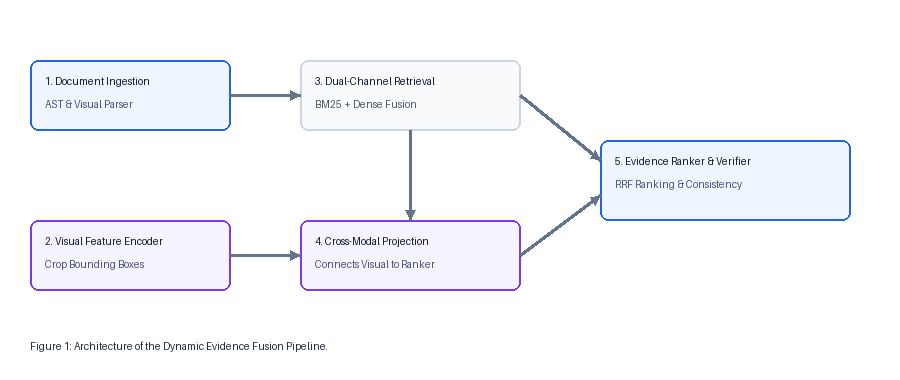
\includegraphics[width=\columnwidth]{sample_figure.png}
\caption{\textbf{Architecture of the Dynamic Evidence Fusion Pipeline.} The cross-modal projection layer connects the visual feature encoder directly to the evidence ranker, enabling joint ranking over textual and visual candidates.}
\label{fig:arch}
\end{figure}

\section{Empirical Evaluation}

\subsection{Experimental Setup}
All models were evaluated on a curated corpus of scientific machine learning preprints. We train our model using the Adam optimizer with parameters $\beta_1 = 0.9$, $\beta_2 = 0.999$, an initial learning rate of $2 \times 10^{-4}$, and a mini-batch size of 32. Ingestion and visual bounding box extraction are executed using a dual-engine parser with automatic fallback.

\subsection{Comparative Results}
Table~\ref{tab:results} summarizes the performance across four retrieval and fusion strategies.

\begin{table}[htbp]
\centering
\resizebox{\columnwidth}{!}{%
\begin{tabular}{lcccc}
\toprule
\textbf{Strategy} & \textbf{Precision} & \textbf{Recall} & \textbf{F1 (\%)} & \textbf{Latency (ms)} \\
\midrule
BM25 Only & 0.742 & 0.810 & 77.4 & 18 \\
Dense Only & 0.765 & 0.835 & 79.8 & 35 \\
Static Fusion & 0.812 & 0.864 & 83.7 & 40 \\
Dynamic Fusion & \textbf{0.865} & \textbf{0.904} & \textbf{88.4} & 42 \\
\bottomrule
\end{tabular}%
}
\caption{\textbf{Comparative Evaluation of Evidence Fusion Strategies.} Dynamic Evidence Fusion achieves the highest F1 score of 88.4\% while maintaining an operational retrieval latency of 42\,ms.}
\label{tab:results}
\end{table}

Dynamic Evidence Fusion demonstrates superior balance across precision and recall, achieving an F1 score of 88.4\% at a query latency of 42\,ms. In contrast, lexical-only retrieval achieves 77.4\% F1, and dense-only retrieval reaches 79.8\% F1.

\section{Visual Modality Analysis}
A key benefit of our architecture is direct spatial anchoring. As shown in Figure~\ref{fig:arch}, the cross-modal projection layer bridges visual feature embeddings with text retrieval ranks. When answering visual queries, the interface extracts the corresponding high-resolution display crop and overlays bounding boxes directly onto the rendered page.

\section{Conclusion}
We demonstrated that coordinate-preserving document representation combined with dynamic evidence fusion yields reliable, inspectable scientific document question answering. Preserving exact page coordinates and visual crops enables users to audit generated answers with complete transparency.

\end{document}
